% Project Management Plan Documentation Template %
% Template made following ISO/IEC/IEEE 16326:2009 %

% Author : Alejandro Muñoz Del Álamo %
% Copyright 2019 %

% Solution Design %

\chapter{Diseño del sistema}
De acuerdo con las decisiones tomadas en el capítulo anterior, hay que tomar una serie de decisiones 
referentes a la forma de elaborar la solución al problema. El primer paso es determinar las herramientas 
con las que se va a implementar la solución: sistemas, lenguajes, APIs, etc. Seguidamente, se presentará 
la arquitectura software del proyecto, que describe los elementos que forman parte del mismo, sus relaciones y
sus interacciones.

\section{Análisis de las herramientas}
En esta sección, se ofrece un estudio del arte de las diferentes alternativas tecnológicas que permitan satisfacer 
los requerimientos del sistema, para optar por una de las opciones planteadas, que será dispuesta como base 
para el software a desarrollar.\medskip

Con este motivo, hemos optado por recoger algunas de las tecnologías existentes para realizar desarrollo de aplicaciones 
móviles.

\subsection{Android Studio}
Android Studio es el entorno de desarrollo integrado (\textit{IDE}) oficial para el desarrollo de apps para Android, 
basado en \textit{IntelliJ IDEA} de \textit{JetBrains} y ha sido publicado gratuitamente a través de la Licencia Apache 2.0.
Disponible para las plataformas \textit{Windows}, \textit{macOS} y \textit{GNU/Linux}. Basado en el lenguanje \textit{Java},
no tiene herramientas nativas para trabajar directamente con \textit{RDF} y \textit{OWL}. Para suplir este obstáculo, 
haríamos uso del framework libre \textit{Apache Jena}, cuya API permite trabajar con RDF, consiguiendo vincular 
el desarrollo en aplicaciones móviles con el uso de ontologías.
% https://es.wikipedia.org/wiki/Android_Studio
% https://jena.apache.org/

\subsection{React Native}
React Native es un \textit{framework} para el desarrollo de aplicaciones móviles de código abierto desarrollado por 
\textit{Facebook}. Se utiliza para desarrollar aplicaciones para \textit{Android}, \textit{iOS}, \textit{Web} y 
\textit{UWP} permitiendo a los desarrolladores usar \textit{React} con funcionalidades nativas de las plataformas.
Al igual que \textit{Android Studio}, React Native no tiene herramientas nativas para el desarrollo de ontologías, de 
manera que haríamos uso de bibliotecas tales como \textit{rdflib.js} para poder proceder al tratamiento de las ontologías.
% https://en.wikipedia.org/wiki/React_Native
% https://github.com/linkeddata/rdflib.js

\subsection{Xamarin}
Xamarin es una plataforma de código abierto para compilar aplicaciones modernas y con mejor rendimiento para \textit{iOS}, 
\textit{Android} y \textit{Windows} con \textbf{.NET}. Xamarin es una capa de abstracción que administra la comunicación 
de código compartido con el código de plataforma subyacente. Xamarin dispone de una biblioteca conocida como 
\textit{RDFSharp}, que permite generar y procesar ontologías en formatos \textit{RDF} y \textit{OWL}.
% https://docs.microsoft.com/es-es/xamarin/get-started/what-is-xamarin
% https://github.com/mdesalvo/RDFSharp


\section{Solución propuesta}
Tras considerar las opciones planteadas en el apartado anterior, se ha considerado descartar \textit{Android Studio} en 
primer lugar, ya que sólo permite el desarrollo en \textit{Android}, mientras que las otras soluciones permiten realizar 
el desarrollo en varias plataformas. \medskip

Una vez desechada una de las opciones, se ha comprobado que las soluciones restantes son compatibles con el proyecto, y 
prácticamente generan el mismo resultado. Por ello, en vez de considerar las plataformas, se ha realizado una comparación 
en función al lenguaje de programación con el que se trabaja en cada una de ellas, que son \textit{\textbf{JavaScript}} en 
\textit{React Native}, y \textit{\textbf{C\#}} para \textit{Xamarin}. Esta comparativa se realizará en forma de tabla.\bigskip

\begin{table}[htb]
\centering
\caption{Comparativa entre \textit{JavaScript} y \textit{C\#}}
\bigskip
\begin{tabular}{|c|c|c|}
    \hline
    & \textit{\textbf{JavaScript}} & \textbf{\textit{C\#}} \\ \hline \hline
    \textbf{Tipo de Lenguaje} & Scripting & Orientado a Objetos \\ \hline
    \textbf{Tipado} & Débil & Fuerte \\ \hline
    \textbf{Detección de errores} & Ejecución & Compilación y ejecución \\ \hline
    \textbf{Compilación} & No & Sí \\ \hline
    \textbf{Mantenibilidad} & Complejo & Sencillo \\ \hline
    \textbf{Soporte de IDE} & No & Microsoft Visual Studio \\ \hline
    \textbf{Sintaxis} & OBSL & OOP \\ \hline
\end{tabular}
\end{table}  


En la comparativa se puede observar que JavaScript es un lenguaje de scripting débilmente tipado que 
no requiere ser compilado, pero resulta difícil de mantener en sistemas complejos. Por otro lado, 
C\# es un lenguaje orientado a objetos fuertemente tipado que requiere ser compilado, que permite 
una mayor facilidad a la hora de mantener el código en sistemas de alta complejidad.

Dado que la aplicación a desarrollar es de una complejidad considerable y que puede ser propensa 
a generar errores, y a la vista de la comparativa mostrada previamente, se ha llegado a la conclusión 
de que la mejor herramienta para el desarrollo del presente proyecto es \textit{\textbf{Xamarin}} con 
la biblioteca \textit{\textbf{RDFSharp}}.

\section{Arquitectura software}
En esta sección se va a describir la arquitectura física y lógica del sistema, especificando su estructura, funcionamiento e 
interacción entre los componentes software.

\subsection{Arquitectura física}
Primero se tendrá que conocer los componentes del dispositivo que serán necesarios para ejecutar el software que se 
va a desarrollar. \medskip

Como el sistema será desarrollado como aplicación móvil multiplataforma, debería poder ejecutarse en \textit{Android} e 
\textit{iOS}, pero debido a que no se dispone del material necesario para realizar el desarrollo en este último, el 
dispositivo tendrá como requisito disponer de \textit{Android} como sistema operativo, siendo la versión 9.0 la más 
reciente cuando se ha realizado el desarrollo.


\subsection{Arquitectura lógica}
Para definir la estructura lógica del sistema, se tomó la decisión de utilizar el patrón de arquitectura software 
\textit{Modelo-Vista-Modelo de Vista} (\textbf{MVVM}), que separa los datos de la lógica de negocio de la interfaz 
de usuario. \textit{MVVM} propone organizar la estructura del software en tres componentes: \textit{modelo}, 
\textit{modelo de vista} y \textit{vista}.
% Poner pie de página aclaración el acrónimo

\begin{itemize}

    \item \textbf{Modelo}: Las clases de modelo son clases no 
    visuales que encapsulan los datos de la aplicación. Por lo tanto, se 
    puede considerar que el modelo representa el modelo de dominio de la 
    aplicación, que normalmente incluye un modelo de datos junto con la 
    lógica de validación y negocios. 
    %https://docs.microsoft.com/es-es/xamarin/xamarin-forms/enterprise-application-patterns/mvvm

    \item \textbf{Modelo de vista}: El modelo de vista implementa las 
    propiedades y los comandos a los que la vista puede enlazarse y notifica 
    a la vista de cualquier cambio de estado a través de los eventos de 
    notificación de cambios. Las propiedades y los comandos que proporciona 
    el modelo de vista definen la funcionalidad que ofrece la interfaz de 
    usuario, pero la vista determina cómo se mostrará esa funcionalidad.
    %https://docs.microsoft.com/es-es/xamarin/xamarin-forms/enterprise-application-patterns/mvvm

    \item \textbf{Vista}: La vista es responsable de definir 
    la estructura, el diseño y la apariencia de lo que el usuario ve 
    en la pantalla. Idealmente, cada vista se define en XAML, con un 
    código subyacente limitado que no contiene la lógica de negocios. 
    Sin embargo, en algunos casos, el código subyacente podría contener 
    lógica de la interfaz de usuario que implementa el comportamiento 
    visual que es difícil de expresar en XAML, como animaciones.
    %https://docs.microsoft.com/es-es/xamarin/xamarin-forms/enterprise-application-patterns/mvvm

\end{itemize}
\bigskip
\begin{figure}[htp]
    \centering
    \label{mvvm}
    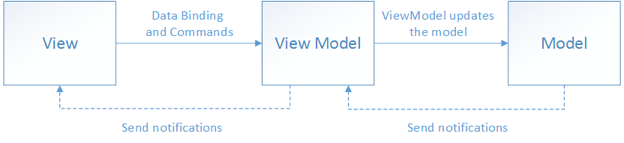
\includegraphics[width=13cm]{Figures/mvvm.png}
    \caption{Patrón Modelo - Vista - Modelo de Vista}
\end{figure}

\subsection{Diseño Lógico de Datos}
En esta sección se debería describir el diseño de la estructura que almacena la información del sistema.
Como no se puede realizar el diseño de una ontología específica, ya que uno de los objetivos de la aplicación 
es generalizar el tratamiento de la información, de manera que se pueda trabajar con la información de juegos 
diferentes sin variar el método de procesamiento, se va a proceder a detallar el diseño general que debe 
tener una ontología para poder ser procesada por la aplicación. \medskip

Para poder describir la estructura requerida por el sistema, se va a emplear a modo de ejemplo la ontología 
que se ha desarrollado simultáneamente con el proyecto y que ha servido para realizar las comprobaciones que aseguran
el correcto funcionamiento de la aplicación, y por tanto, sigue esta estructura. \medskip

% 1º - Explicar ONTOLOGÍAS AQUÍ
% 2º - Explicar Estructura Ontología 
% 3er - Explicar Jerarquia de información
% 4º - Anotaciones
% 4.1 Anotaciones estándar
% 4.2 Anotaciones personalizadas



